\documentclass{article}
\usepackage[landscape]{geometry}
\usepackage{url}
\usepackage{multicol}
\usepackage{amsmath}
\usepackage{esint}
\usepackage{amsfonts}
\usepackage{tikz}
\usetikzlibrary{decorations.pathmorphing}
\usepackage{amsmath,amssymb}

\usepackage{colortbl}
\usepackage{xcolor}
\usepackage{mathtools}
\usepackage{amsmath,amssymb}
\usepackage{enumitem}
\usepackage{tcolorbox}
\makeatletter

\newcommand*\bigcdot{\mathpalette\bigcdot@{.5}}
\newcommand*\bigcdot@[2]{\mathbin{\vcenter{\hbox{\scalebox{#2}{$\m@th#1\bullet$}}}}}
\makeatother

\title{STAT 251 Formula Sheet}
\usepackage[brazilian]{babel}
\usepackage[utf8]{inputenc}

\advance\topmargin-.8in
\advance\textheight3in
\advance\textwidth3in
\advance\oddsidemargin-1.45in
\advance\evensidemargin-1.45in
\parindent0pt
\parskip2pt
\newcommand{\hr}{\centerline{\rule{3.5in}{1pt}}}
%\colorbox[HTML]{e4e4e4}{\makebox[\textwidth-2\fboxsep][l]{texto}

\begin{document}

\begin{center}{\huge{\textbf{UAI Formula Sheet}}}\\
\end{center}
\begin{multicols*}{2}

\tikzstyle{mybox} = [draw=black, fill=white, very thick,
    rectangle, rounded corners, inner sep=5pt, inner ysep=10pt]
\tikzstyle{fancytitle} =[fill=black, text=white, font=\bfseries]
%% ---- 0. Handy Theorems ----
% --- Handy Theorems 
\begin{tikzpicture}
    \node [mybox] (box){%
        \begin{minipage}{0.48\textwidth}
        \begin{tabular}{lp{0.48\textwidth} l}

            % --- Handy Theorems ---
            Chain Rule:
            &
            $P(X_1, X_2) = P(X_1 | X_2) P(X_2)$
            
            \\
            
            Marginalization:
            &
            $P(X_1) = \sum_{x \in X_2} P(X_1, X_2 = x)$
            
            \\
            
            Bayes Rule:
            &
            $P(X_1 | X_2) = \frac{P(X_2 | X_1) P(X_1)}{P(X_2)}$
            
            \\

            1.
            &
            $P(X_1 | X_2) = \frac{P(X_2 | X_1) \cdot P(X_1)}{
                \sum_{x \in X_1} P(X_2 | X_1 = x) \cdot P(X_1 = x)
            }$

            \\
            
            2. &
            $P(X_1 | X_2, X_3) = \frac{P(X_2 | X_1, X_3) \cdot P(X_1 | X_3)}{P(X_2 | X_3)}$
            
            \\
            
            3. &
            $P(X_1 = x | X_2) = \frac{P(X_2 | X_1 = x) \cdot P(X_1 = x)}{P(X_2)}$
        \end{tabular}
    \end{minipage}
};
%------------ Handy Theorems Header ---------------------
\node[fancytitle, right=10pt] at (box.north west) {Handy Theorems};
\end{tikzpicture}

%% ---- 1. Bayesan Networks ----
% --- Bayesan Networks ---
\begin{tikzpicture}
    \node [mybox] (box)
    {%
        \begin{minipage}{0.48\textwidth}
        \begin{tabular}{lp{0.48\textwidth} l}
            % --- Bayesan Networks ---
            Bayesan Network:
            &
            a DAG where Nodes represent random variables and edges represent direct influence.

            \begin{tikzpicture}
                \node (X_1) at (0,0) {Cloudy};
                \node (X_2) at (-1.5,-1.5) {Sprinkler};
                \node (X_3) at (1.5,-1.5) {Rain};
                \node (X_4) at (0,-3) {WetGrass};

            \draw[->](X_1)--(X_2);
            \draw[->](X_1)--(X_3);
            \draw[->](X_2)--(X_4);
            \draw[->](X_3)--(X_4);
            \end{tikzpicture}
            \\

            % -- Conditional Independence ---
            Conditional Independence:
            &
            $P(X_1 | X_2, X_3) = P(X_1 | X_3)$

            then $X_1$ and $X_2$ are conditionally independent given $X_3$

            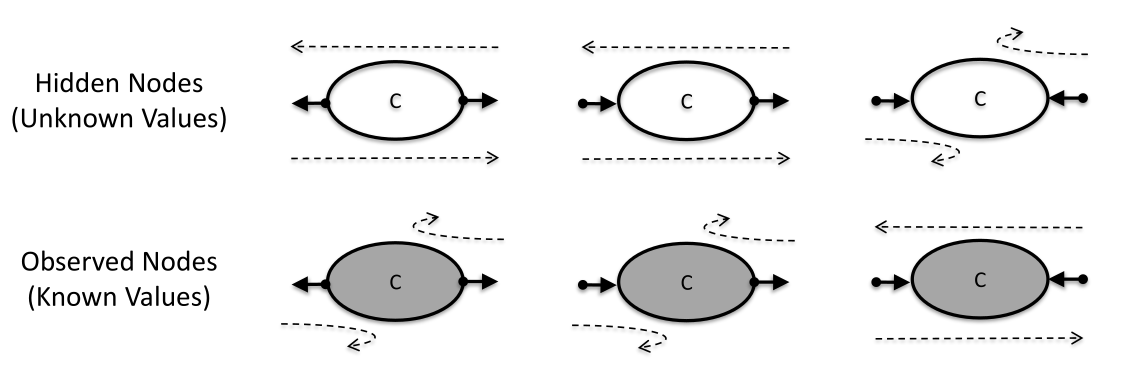
\includegraphics[width=0.48\textwidth]{imgs/01_conditional_indipendence.png}
            
            Two (sets of) nodes $A$ and $B$ are conditionally independent (d-separated) given $C$ if and only if all the path from $A$ to $B$ are shielded by $C$.

            \\

            % --- Joint Distribution Factorization ---
            Joint Distribution Factorization:
            &
            $P(X_1,\ldots, X_n) = \prod_{i=1}^{n} P(X_i | \text{pa}(X_i))$

            \\

            % --- Explaining Away ---
            Explaining Away:
            &
            describes two variable which become dependent because you observe a third one.
        \end{tabular}

        \end{minipage}
    };

%------------ Bayesan Networks Header ---------------------
\node[fancytitle, right=10pt] at (box.north west) {Bayesan Networks};
\end{tikzpicture}
% ----- Dynamic Bayesian Networks -----
%------------ Dynamic Bayesian Networks ---------------
\begin{tikzpicture}
    \node [mybox] (box){%
        \begin{minipage}{0.48\textwidth}
        \begin{tabular}{lp{0.48\textwidth} l}
            % --- Markov Chain ---
            (first Order) Markov Chain:
            & $P(X_{t+1} | X_t, X_{t-1}, ..., X_1) = P(X_{t+1} | X_t)
            $

            \\

            % --- Stationary Event ---
            Stationary Event:
            & $P(X_{t+1} = j| X_t = i) = p_{ij} \ \forall t$ 
            
            \\

            % --- Transition Matrix ---
            Transition Matrix:
            &  $P = \begin{bmatrix} p_{11} & ... & p_{1n} \\ ... & ... & ... \\ p_{n1} & ... & p_{nn} \end{bmatrix}$ \
            $\sum_{j=1}^{n} p_{ij} = 1$ 
            
            \\

            % --- Probability at step n ---
            Probability at step n:
            & $P_{ij}(n) = P^n(i,j)$ 
            
            \\

            % --- Definitions ---
            Reachability:
            & A state $j$ is reachable from $i$ if there exists a path from $i$ to $j$ \\

            Communicability:
            & States $i$ and $j$ communicate if each is reachable from the other \\

            Absorbing State:
            & A state $i$ is absorbing if $p_{ii} = 1$ \\

            Transient State:
            & A state $i$ is transient if it is reachable from another state $j$ but not vice versa. \\

            Recurrent State:
            & A state $i$ is recurrent if it is not transient. \\

            Ergodic Markov Chain:
            & A Markov Chain is ergodic if it is:
            
            \begin{itemize}[label={--}, topsep=0cm, parsep=0cm, itemsep=0cm]
                \item Recurrent
                \item Aperiodic
                \item All states communicate
            \end{itemize} 
            
            \\

            % --- Steady State Distribution ---
            Steady State Distribution:
            & $\pi = \lim_{n \to \infty} P^n$ 
            
            \\

            % --- Expected Transient Time ---
            Expected Transient Time:
            & $m_{ij} = 1 + \sum_{k \neq j} p_{ik} m_{kj}$ 
            
            \\

            % --- Absorbing Markov Chain ---
            Absorbing Markov Chain:
            & $P = \begin{bmatrix} Q & R \\ 0 & 1 \end{bmatrix}$ \
            $Q$ transient states, $R$ absorbing states.

        \end{tabular}
        \end{minipage}
    };
    %------------ Dynamic Bayesian Networks Header ---------------------
    \node[fancytitle, right=10pt] at (box.north west) {Markov Chains};
    \end{tikzpicture}
% --- Hidden Markov Models 
\begin{tikzpicture}
    \node [mybox] (box){%
        \begin{minipage}{0.48\textwidth}
        \begin{tabular}{lp{0.48\textwidth} l}

            % --- Hidden Markov Models ---
            Hidden Markov Models:
            &
            A HMM is $(S, E, P, A, B)$:
            \begin{itemize}[label={--}, topsep=0cm, parsep=0cm, itemsep=0cm]
                \item $S$ is the set of hidden states
                \item $E$ is the set of observations
                \item $P$ is the distribution of the initial state
                \item $A$ is the transition probability matrix
                \item $B$ emission probability matrix
            \end{itemize}

            \\
        \end{tabular}
    \end{minipage}
};
%------------ Hidden Markov Models Header ---------------------
\node[fancytitle, right=10pt] at (box.north west) {Hidden Markov Models};
\end{tikzpicture}


% --- Viterbi Algorithm ---
\begin{tikzpicture}
    \node [mybox] (box){%
        \begin{minipage}{0.48\textwidth}
            \begin{paragraph}
                From observations, compute the most likely sequence of hidden states:
                \begin{equation}
                    \arg \max P(X_{1:t} | e_{1:t}) = 
                    \arg \max \frac{P(X_{1:t}, e_{1:t})}{P(e_{1:t})} = 
                    \arg \max P(X_{1:t}, e_{1:t})
                \end{equation}

                Lets apply bayesan factorization:
                \begin{equation}
                    P(X_{1:t}, e_{1:t}) = P(X_0) \prod_{i=1}^{t} P(X_i | X_{i-1}) P(e_i | X_i)
                \end{equation}

                The solution is the one that minimize:
                \begin{equation}
                    - \log P(X_{1:t}, e_{1:t}) = 
                    - \log P(X_0) + \sum_{i=1}^{t} 
                    (- \log P(X_i | X_{i-1}) - \log P(e_i | X_i))
                \end{equation}
            \end{paragraph}
            \begin{tcolorbox}[colback=gray!5, colframe=gray!80!black, title={Graph Construction}] 
                Construct a graph with $1 + t \cdot n$ nodes, where $n$ is the number of hidden states with one initial node and $n$ nodes at time $i$ where $j^{th}$ node is $X_i = s_j$.

                Find the shortest path from the initial node to the final node considering the weights of the edges.
                
                %--- Graph Construction ---
                \begin{center}
                \begin{tikzpicture}
                    % Define nodes
                    \node (X_0) at (0,0) {$X_0$};
                    \node (X_1) at (3,1) {$X_1$};
                    \node (X_2) at (3,0) {$X_2$};
                    \node (X_3) at (3,-1) {$X_3$};
                    \node (X_11) at (6,2) {$X_{11}$};
                    \node (X_12) at (6,0) {$X_{12}$};
                    \node (X_13) at (6,-2) {$X_{13}$};
                    \node (X_21) at (9,2) {$X_{21}$};
                    \node (X_22) at (9,0) {$X_{22}$};
                    \node (X_23) at (9,-2) {$X_{23}$};
                    % Add indices to the states
                    \node at (0, 3) {0};
                    \node at (3, 3) {1};
                    \node at (6, 3) {2};
                    \node at (9, 3) {3};
                    % Draw edges
                    \draw (X_0) -- node[above, font=\scriptsize, rotate=20] {$-\log P(X_0 = 1)$} (X_1);
                    \draw (X_0) -- (X_2);
                    \draw (X_0) -- (X_3);
                    \draw (X_1) -- (X_11);
                    \draw (X_1) -- (X_12);
                    \draw (X_1) -- (X_13);
                    \draw (X_2) -- (X_11);
                    \draw (X_2) -- (X_12);
                    \draw (X_2) -- (X_13);
                    \draw (X_3) -- (X_11);
                    \draw (X_3) -- (X_12);
                    \draw (X_3) -- node[below, font=\scriptsize, rotate=-20] {$-\log P(X_3 | X_3) \ - \log P(e_t | X_3)$} (X_13);
                    \draw (X_11) -- (X_21);
                    \draw (X_11) -- (X_22);
                    \draw (X_11) -- (X_23);
                    \draw (X_12) -- (X_21);
                    \draw (X_12) -- (X_22);
                    \draw (X_12) -- (X_23);
                    \draw (X_13) -- (X_21);
                    \draw (X_13) -- (X_22);
                    \draw (X_13) -- (X_23);
    
                \end{tikzpicture}
                \end{center}
            \end{tcolorbox}
        \end{minipage}
};
%------------ Viterbi Algorithm Header ---------------------
\node[fancytitle, right=10pt] at (box.north west) {HMM: Viterbi Algorithm};
\end{tikzpicture}

\end{multicols*}
\end{document}


Contact GitHub API Training Shop Blog About
© 2016 GitHub, Inc. Terms Privacy Security Status Help